\documentclass{beamer}
\usepackage[utf8x]{inputenc}
\usepackage{hyperref}
\usepackage[footheight=1em]{beamerthemeboxes}
\usepackage{listings}
\usepackage{ulem}
\usepackage{color}
%\usepackage{pgfpages}
%\setbeameroption{show notes on second screen=left}
\usetheme{Singapore}


\setbeamertemplate{footline}{
\leavevmode%
\hbox{
\hspace*{-0.06cm}
\begin{beamercolorbox}[wd=.8\paperwidth,dp=1ex,left]{section in head/foot}%
	\usebeamerfont{section in head/foot}
\end{beamercolorbox}%
\begin{beamercolorbox}[wd=.2\paperwidth,ht=2.25ex,dp=1ex,right]{section in head/foot}%
	\insertframenumber{}\hspace*{2ex}
\end{beamercolorbox}}%
\vskip0pt%
}

\setbeamertemplate{navigation symbols}{}

%\usetheme{Frankfurt}


%\addfootboxtemplate{\color{white}}{\color{gray}
  %\insertframenumber/\inserttotalframenumber\null}



\setbeamertemplate{background canvas}{
\includegraphics
   [width=\paperwidth,height=\paperheight]{files/fond.png}}


\title{Metadata graph}
\author{Thibaut \textsc{Marmin} \and Namrata \textsc{Patel} \\ Clément \textsc{Sipieter}}
\institute{Projet Gestion de données distribuées GMIN210 : génération de graphes à partir des métadonnées.\\\texttt{https://github.com/marminthibaut/graph\_database/}}
\date{11 Mai 2012}

\begin{document}

% Def variable coloration code source
\definecolor{keyword}{rgb}{0.55,0,0} 
\definecolor{type}{rgb}{0,0.55,0} 
\definecolor{comment}{rgb}{0.7,0.7,0.7} 

\lstset{
basicstyle=\footnotesize\sffamily,
numbers=none,
numberstyle=\footnotesize\color{comment},
keywordstyle=\color{keyword}\bfseries,
commentstyle=\color{comment},
breaklines=true,
fontadjust=true,
columns=fullflexible,
morekeywords=true
}

\AtBeginSection[]
{
  \begin{frame}{Metadata graph}
  \begin{columns}[t]
  \begin{column}{5cm}
  \tableofcontents[sections={1-3},currentsection,hideothersubsections]
  \end{column}
  \begin{column}{5cm}
  \tableofcontents[sections={4-6},currentsection,hideothersubsections]
  \end{column}
  \end{columns}
  \end{frame}
}

\begin{frame}
\titlepage
\end{frame}

\begin{frame}{Metadata graph}
    

  \begin{columns}[t]
  \begin{column}{5cm}
  \tableofcontents[sections={1-3},hideallsubsections]
  \end{column}
  \begin{column}{5cm}
  \tableofcontents[sections={4-6},hideallsubsections]
  \end{column}
  \end{columns}

\end{frame}

\section{Besoins}
\subsection{Fonctionnalités}
\begin{frame}{Besoins}{Fonctionnalités}

\end{frame}

\subsection{Contraintes}
\begin{frame}{Besoins}{Contraintes}

\end{frame}

\section{Conception}
\textit{Cette phase d'analyse est un élément indispensable à la bonne réalisation du projet. Dans un premier temps, un modèle plus fidèle à la réalité des schémas stockés dans les SGBDR est présenté. Cette partie est suivit d'une petite réflexion sur l'utilisation des ORM. Sont ensuite parcourus les solutions de génération de graphes pour la représentation des données. Les choic concernant l'interface utilisateur seront également exposés.}

\section{Le modèle}
\subsection{Modèle réellement rencontré}

Lors de l'étude des métadonnées stockées par les différents SGBD, nous avons remarqué quelque divergences par rapport au modèle fournit avec le sujet (figure~\ref{figure:diag_classe_fournit} page~\pageref{figure:diag_classe_fournit}). La figure~\ref{figure:diag_classe_reel} présente un diagramme de classe construit suite à nos recherches.

\begin{figure}[H]
\centering
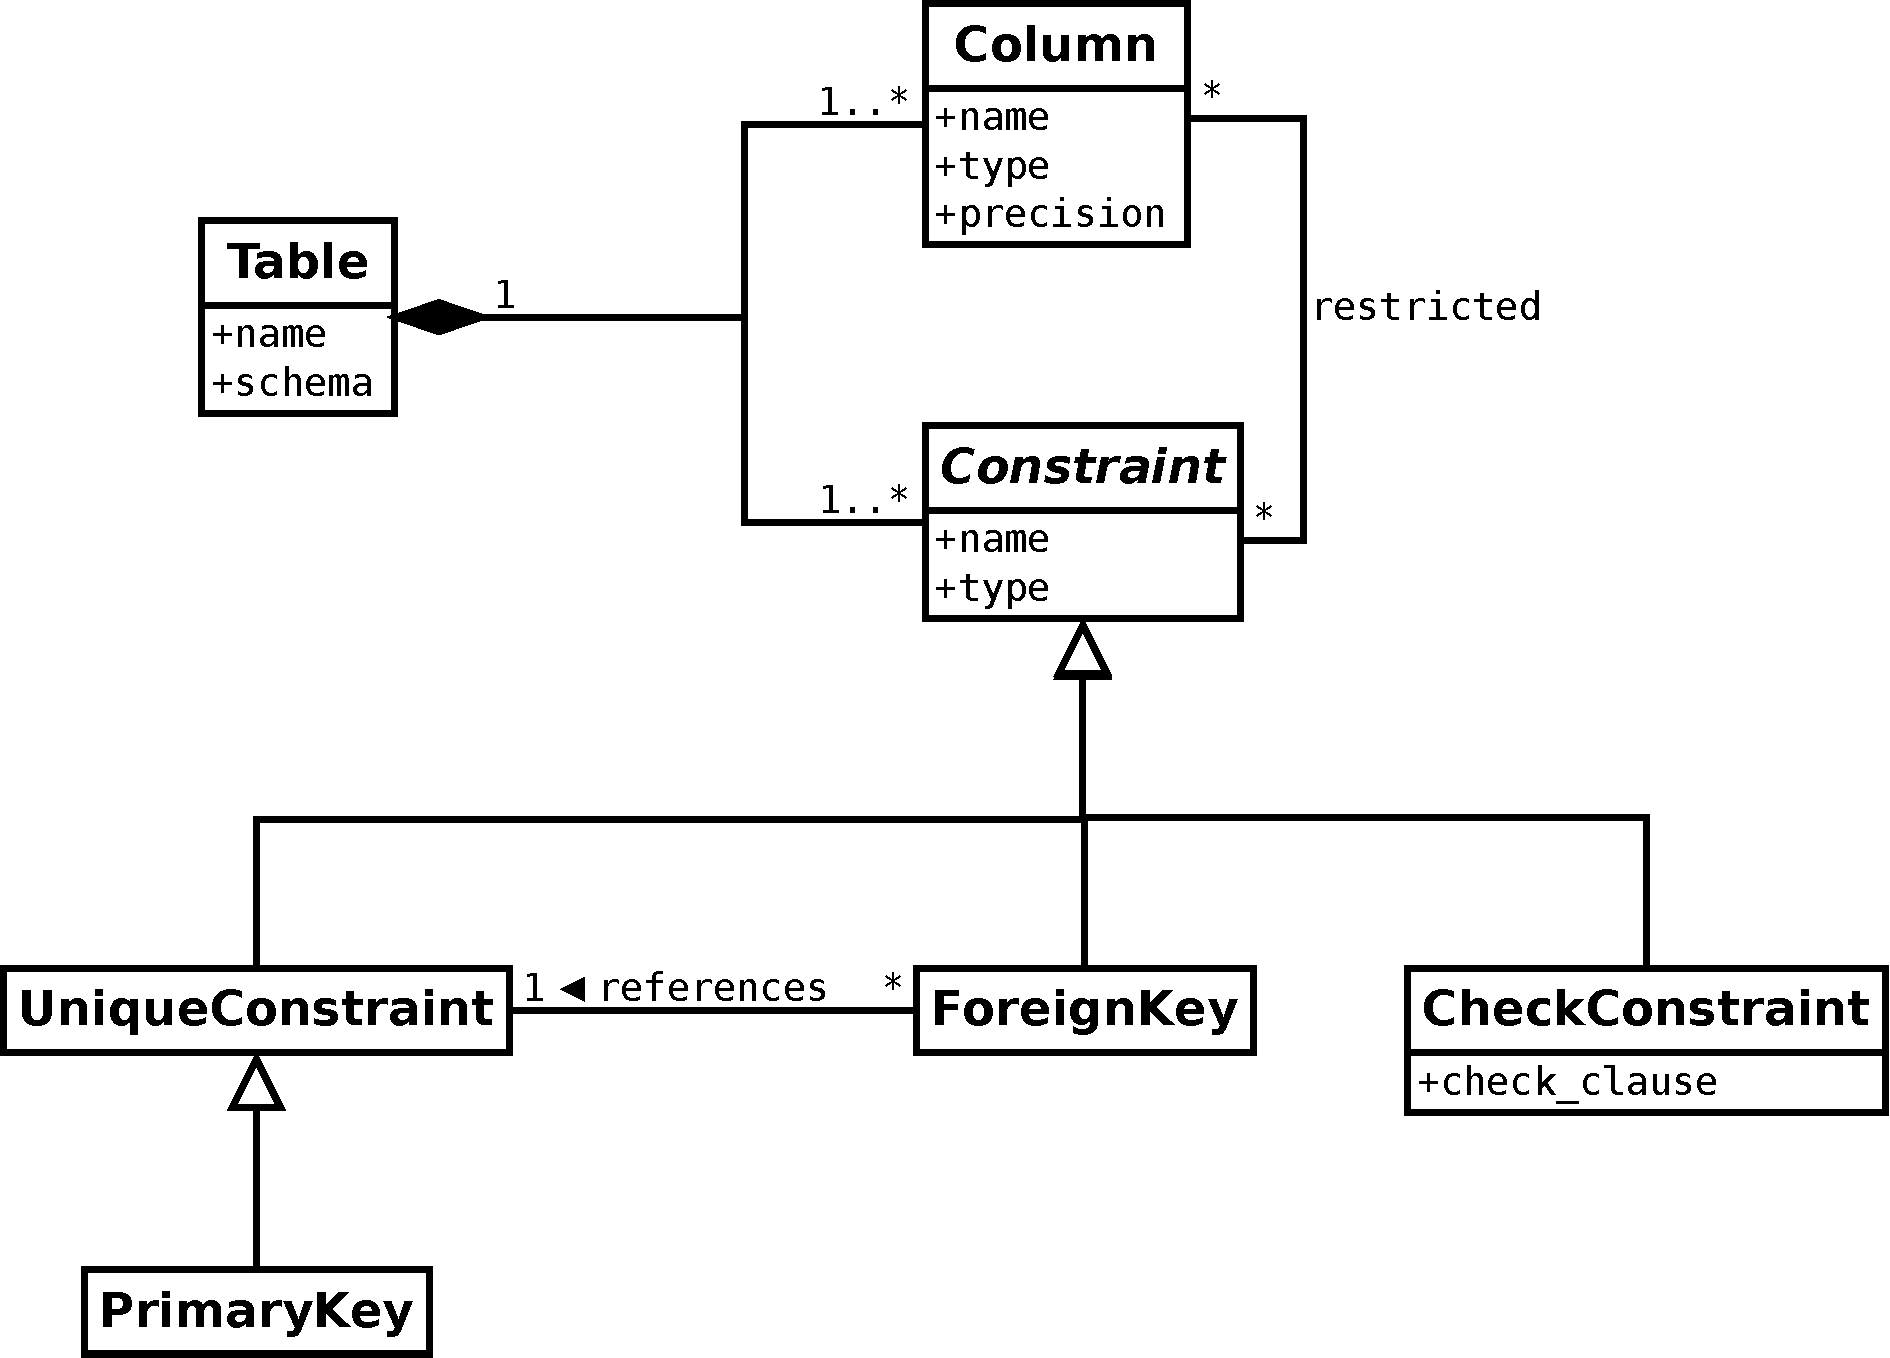
\includegraphics[width=\textwidth]{files/diag_class_ameliore}
\caption{Diagramme de classe réellement rencontré.}
\label{figure:diag_classe_reel}
\end{figure}

La principale différence réside dans la classification des contraintes. Cette classification permet de distinguer trois types de contraintes :

\begin{itemize}
\item Les contraintes d'unicité : elles contraignent l'unicité d'un ou plusieurs attributs au sein d'une même table. Les contraintes de clé primaire sont des contraintes d'unicité.
\item Les contraintes d'intégrité référentielle : elles identifient un ou plusieurs attributs d'une table comme référençant un ou plusieurs attributs d'une autre table, au travers d'une contrainte d'unicité. Notons que ce type de contrainte permet de \textbf{référencer une contrainte d'unicité et non plus une contrainte de clé primaire} comme proposé dans le modèle original.
\item Les contraintes de type \emph{Check} : qui s'appliquent à un ou plusieurs attributs d'une table. Elles contiennent une clause de vérification \texttt{check\_clause}.
\end{itemize}

\paragraph*{NB}
Les contraintes de type \emph{NULL}, \emph{NOT NULL} et \emph{DEFAULT} sont ignorées.

	\subsection{Attributs}
		Gestion des types génériques
	\subsection{Tables}
	\subsection{Contraintes}
	
\section{ORM}
\subsection{Qu'est-ce qu'un ORM ?}
\subsection{Pourquoi ?}

\section{Compatibilité avec les SGBD}

\section{Générateur de graphes}
  \subsection{différentes librairies}
		\paragraph{jung}
				entrée : un fichier dot\\
				inconvénients : dernières fonctionnalités dot non prise en charqe.
		\paragraph{grappa}
				 entrée : fichier dot
		\paragraph{graphviz}
			GraphViz est un ensemble de logiciel libre développé par AT\&T pour la visualisation de graphes. Il introduit le langage de description de graphe DOT.
				
  \subsection{Notre choix}
		\verb+//Notre choix c'est porté sur la commande DOT fournit par GraphViz+

\section{L'IHM}	
	\subsection{les choix possibles}
	\label{ihm_choix_possibles}
		Concernant la conception de l'interface utilisateur, deux choix principaux s'offrent à nous. Le premier est de concevoir
une interface graphique proposant une fenêtre de configuration puis un affichage du résultat obtenu. Le second est de concevoir 	une interface en ligne de commande générant une image. 	
	
		\subsubsection{GUI : \og Graphical User Interface \fg{}}
			Une interface utilisateur graphique permet une prise en main rapide et intuitive d'un logiciel mais ne permet pas une grande interopérabilité. En effet, il est compliqué de demandé à un programme de configurer un autre programme via une interface graphique.
			
		\subsubsection{CLI : \og Command Line Interface \fg{}}
			La conception d'une interface en ligne de commande entre dans la philosophie KISS, « Keep it simple, Stupid! ». Cette philosophie préconise la recherche de simplicité dans la conception et insiste sur le fait que toute complexité non nécessaire devrait être évitée. Cette vision à l'avantage d'offrir une grande interopérabilité, il est en effet aisé d'exécuter une ligne de commande depuis un logiciel et d'en récupérer la sortie. Par contre, une interface en ligne de commande est plus difficile à prendre en main pour un utilisateur non averti.  
			
	\subsection{Notre choix}
		Nous avons choisi pour notre logiciel, d'implémenter une interface en ligne de commande pour les avantages de cette vision, détaillés précédement en \ref{ihm_choix_possibles}, à savoir sa simplicité et sa grande interopérabilité. De plus, nous pouvons, à partir d'une interface en ligne de commande, créer une interface graphique dans un langage quelconque qui encapsule notre logiciel, alors que l'inverse est bien entendu beaucoup moins évident.



\section{Implementation}
\textit{Cette partie présente \emph{Hibernate}, l'ORM que nous avons du utiliser pour gérer l'accès aux données. Elle détaille également les différents paquets de l'application, la manière dont ont été mappé les informations, celle adoptée pour la génération du graphe, ainsi que l'utilisation de l'outil développé en ligne de commande. Notons que l'utilisation du langage Java ne sera pas justifié étant donné qu'il s'agit d'une contrainte induite pas le fait que le framework \emph{Hibernate} devait être utilisé.}

\section{L'ORM \emph{Hibernate}}
\emph{Hibernate} est un framework Java de type ORM. Bien qu'il permette la gestion de la persistance des données (écriture), \emph{Hibernate} sera utilisé ici uniquement dans le but d'accéder aux métadonnées des SGBD (lecture) via des configurations de Mapping.
\subsection{POJO}
La définition des entités dans \emph{Hibernate} à l'aide de classes \emph{POJO}. Cet acronyme signifiant \og Plain Old Java Object \fg{} fait référence à de simples classes ayant comme principale caractéristique de n'implémenter aucune interface, et de posséder un \emph{getter} et un \emph{setter} par attribut.
\subsection{Mapping}
Le mapping consiste, comme son nom l'indique, à faire la correspondance entre les entités définies (classes \emph{POJO}) et les tables en base de données. En règle générale, un objet $x$ est mappé avec une table relationnelle $table-x$, est les attributs $x_1$, $x_2$, \ldots, $x_n$ avec les attributs $tables-x.x_1$, $tables-x.x_1$, \ldots, $tables-x.x_1$. Il est également possible d'ajouter des relations entre attributs (One-to-One, One-to-Many, Many-to-Many), de déclarer des \emph{id}, etc.

\emph{Hibernate} permet de définir le mapping via des annotations directement au sein des classes, ou via des fichiers de configuration xml \texttt{hbm}. C'est cette deuxième méthode que nous avons choisie, et qui sera décrite dans la partie~\ref{section:structure_de_lapplication}.
\subsection{Subselect}

\subparagraph{\ldots}

\section{Structure de l'application}
\label{section:structure_de_lapplication}

Dans le but de faciliter la réutilisation du code et l'extension de sa compatibilité avec de nouveaux SGBDR, nous avons pris soin de structurer l'application. La figure~\ref{figure:structure_appli} présente l'arborescence des paquets Java.

\begin{figure}[H]
\centering
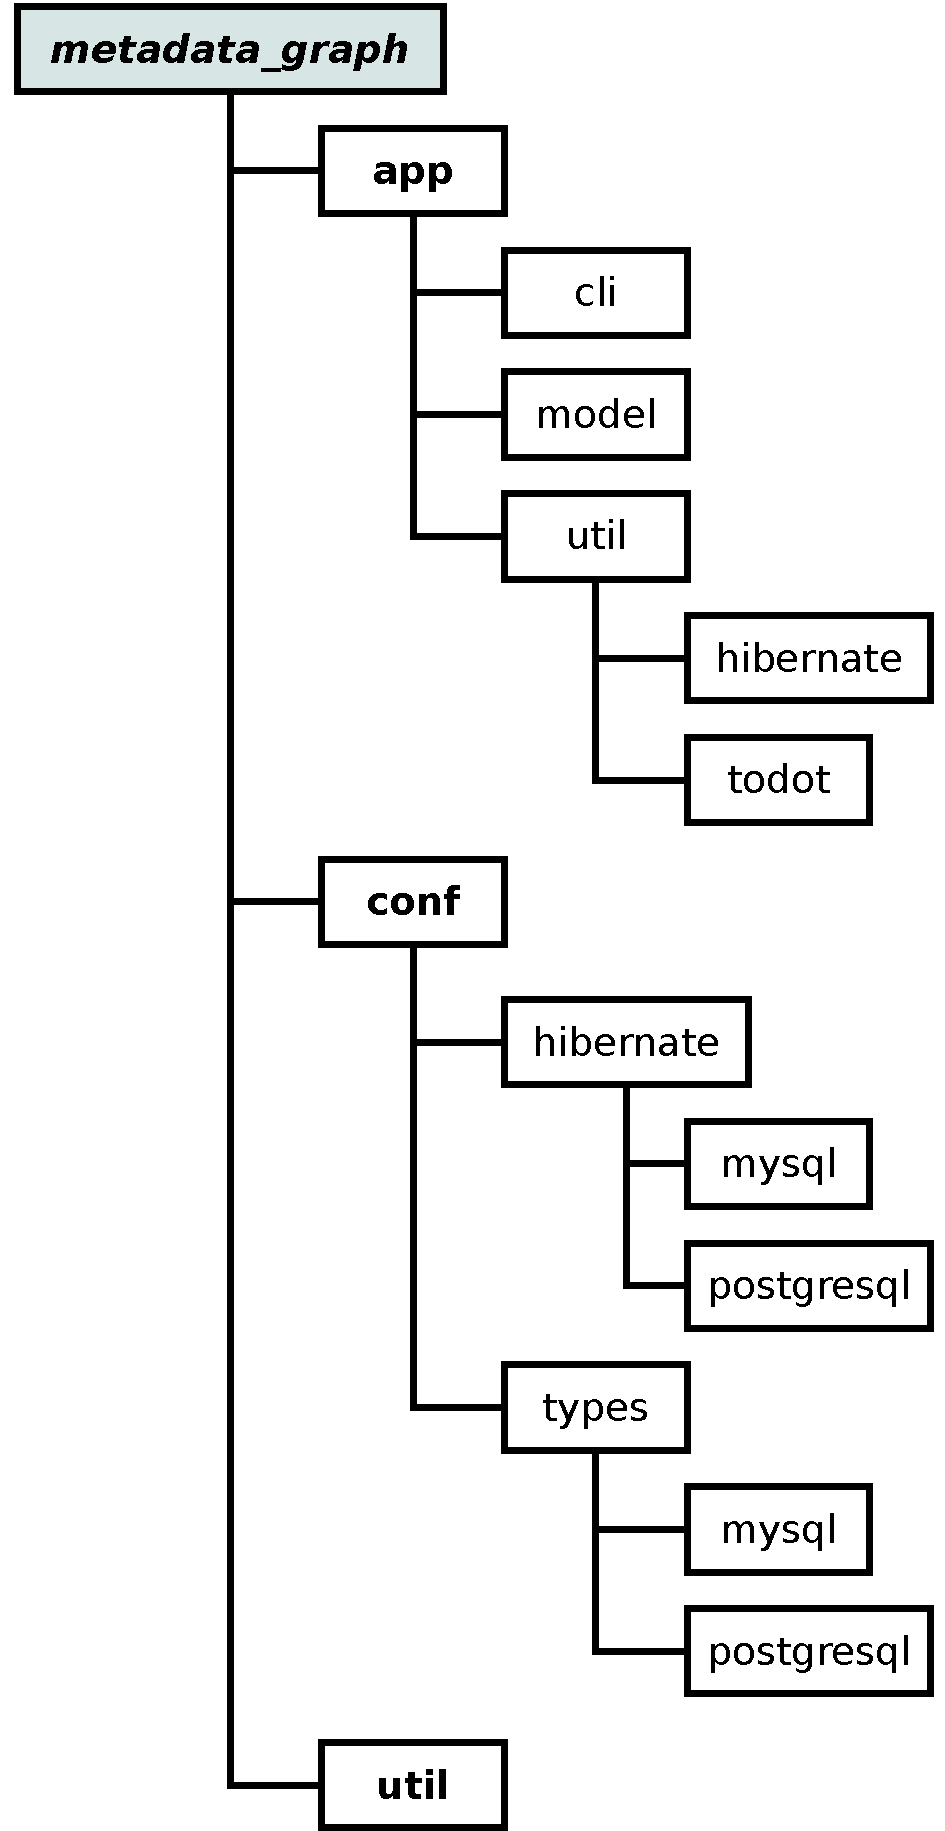
\includegraphics[width=0.5\textwidth]{files/archi}
\caption{Arborescence des paquets Java de l'application.}
\label{figure:structure_appli}
\end{figure}

Trois paquets principaux se distinguent :

\begin{description}
\item[\texttt{app}] : dans ce paquet sont regroupés toutes les classes Java nécessaires au fonctionnement interne de l'outil. On y trouve les sous paquets \texttt{cli}, \texttt{model} et \texttt{util} qui seront détaillés par la suite.
\item[\texttt{conf}] : ce paquet permet d'externaliser les fichiers de configuration. Il a la particularité de ne stocker aucune classe Java.
\item[\texttt{util}] : ici sont regroupés des classes java utilisées par l'application mais qui ne sont pas propre à l'exécution de ses fonctions initiales. Elle stocke notamment des classes permettant la gestion du CLI.
\end{description}

\subsection{Paquet \texttt{app.cli}}

Ce paquet implémente l'interface en ligne de commande, celle-ci permettra notamment la configuration de la connexion au SGBDR ainsi que le format de sortie. Il est composé exclusivement de la classe \texttt{CommandLineInterface}.

\begin{description}
\item[CommandLineInterface] Cette classe défini la fonction \texttt{main} de notre application. Elle utilise la classe \texttt{OptionManager} décrite en \ref{subsection:util} page \pageref{subsection:util} afin d'interpréter les options de la ligne de commande.  
\end{description}

\begin{verbatim}
Usage:
gd SGBD_NAME DATABASE_NAME [OPTION]...

Options:
    -u, --user <USERNAME>
        use this username.
    -p, --password [PASSWORD]
        use this password.
    -h, --host <HOST>
        use this host.
    --port <PORT>
        use this port.
    -o, --output <FILE_NAME>
        generate a png image with graphviz
    -T, --type <type>
        the output format : svg, ps, png, gif, dia… 
        See graphviz output formats for more formats.
    -c, --cmd <GRAPHVIZ_CMD>
        choose your graphviz command (man graphviz).
    --show 
        open a window with graph representation.
    --help
        print this message.
\end{verbatim}


\subsection{Paquet \texttt{app.model}}
C'est ici que sont définies les classes \emph{POJO} du modèle de données correspondant au modèle relationnel. On y trouve donc les classes \texttt{Column}, \texttt{Constraint} et \texttt{Table}, enrichies de quelques méthodes :

\begin{description}

\item[Column] Ajout d'un méthode \texttt{\underline{bool isPk()}} permettant de savoir si la colonne est inclue dans la clé primaire de la table à laquelle elle appartient. Est également définie une méthode \texttt{\underline{String getGenericType()}} qui retourne, sous la forme d'une chaine de caractères, le type générique de la colonne.

\item[Constraint] Ajout des méthodes \texttt{\underline{bool isPk()}}, \texttt{\underline{bool isFk()}} et \texttt{\underline{bool isCheck()}} permettant de savoir respectivement si la contrainte est de type clé primaire, clé étrangère, ou contrainte de vérification. Est également définie une méthode \texttt{\underline{String getGenericType()}} qui retourne, sous la forme d'une chaine de caractères, le type générique de la contrainte.
\end{description}

Les types génériques sont définies dans les énumérations \texttt{ColumnType} et \texttt{ConstraintType}. Les conversions de types se font en fonction du SGBDR sélectionné grâce au paquet \texttt{app.util} (cf. \ref{subsection:app.util}) et aux fichiers de conversions stockés dans le paquet \texttt{conf.types} (cf. \ref{subsection:conf.types}).

\subsection{Paquet \texttt{app.util}}
\label{subsection:app.util}

Des classes utilitaires sont définies dans ce paquet.

\subsubsection{Génération de graphe avec \texttt{ToDotUtil}}
\label{section:ToDotUtil}
Cet utilitaire est définit dans un sous paquet \texttt{todot}. Il contient une succession d'énumérations permettant de lister les commandes \emph{graphviz}, les couleurs, les formes, et les styles propres au langage DOT.
La classe principale \texttt{ToDotUtil} implémente une méthode permettant, à partir d'une base de données (liste de tables), de générer une chaine de caractères au langage DOT qui décrit cette base de données. Il est possible de définir le style du graphe généré en sortie (couleurs, formes, etc.).

Les formats d'exportation suivant sont reconnus : 

\begin{center}
\begin{tabular}{c c c c c c}
canon&cmap&cmapx&cmapx\_np&dot&eps \\
fig & gd & gd2 & gif & gv & imap \\
imap\_np & ismap & jpe & jpeg & jpg & pdf \\
plain & plain-ext & png & ps & ps2 & svg \\
svgz & tk & vml & vmlz & vrml & wbmp \\
x11 & xdot & xlib & & & \\
\end{tabular}
\end{center}

\subsubsection{Singleton de connexion Hibernate}
Le sous paquet \texttt{hibernate} contient une classe \texttt{HibernateUtil} respectant le patron de conception \emph{singleton}. Il permet de créer une session \emph{Hibernate} en fournissant le type de SGBD, l'hôte, le nom de la base de données, le nom d'utilisateur, le mot de passe et le port.

La création de la session s'effectue en chargeant le fichier de configuration \emph{Hibernate} correspondant au type de SGBD passé en paramètre, et renvoie une exception si celui-ci est inexistant ou inaccessible.

\subsubsection{Types génériques}
Comme décrit dans la section~\ref{section:generic_types}, nous avons fait le choix de généraliser les types de colonnes et de contraintes. Cette classe utilitaire fournit une unique méthode permettant, à partir du type de SGBD, du type non générique, et du type d'objet (colonne ou contrainte), de retourner le type générique. La méthode procède en chargeant le fichier de correspondance des types du SGBD passé en paramètre. Ces fichiers sont décrits dans la section~\ref{subsection:conf.types}.

\subsection{Paquet \texttt{conf.hibernate}}
Les fichiers de configurations d'\emph{Hibernate} propre à chaque SGBDR sont stockés ici. Il faut créer un sous paquet au nom du SGBDR (en respectant le nom du driver JDBC).

Chaque SGBDR doit posséder quatre fichiers de configuration. La configuration principale déclare le driver et le dialecte à utiliser, ainsi que les chemin vers les trois fichiers de Mapping décrits ci-après.
\subsubsection{Fichiers de mapping}
\paragraph{Le \emph{subselect}} Le subselect permet d'associer non pas une entité du modèle à une table réellement stockée en  base de données, mais à un table virtuelle créée via un requête de sélection. Nous avons donc pu généraliser notre modèle de données en adaptant les clauses \emph{subselect} pour chaque SGBD, afin de sélectionner, à partir des vues proposées par les différents systèmes, les données nécessaires.

\paragraph{Problématique de la relation \emph{Many-to-Many}}
Lors de la construction de nos fichiers de mapping, nous avons rencontré un problème au niveau du modèle de données auquel nous étions confrontés (cf. figure~\ref{figure:diag_classe_reel}, page \pageref{figure:diag_classe_reel}). D'après ce modèle, l'entité contrainte est en relation \emph{Many-to-Many} avec l'entité colonne. Dans le modèle relationnel, une telle relation nécessite la création d'une table d'association, permettant la jointure entre ces deux entités. Étant donné que nous travaillons avec des \emph{subselect}, nous ne pouvons pas créer de telle table. La solution a donc consisté en adaptant le schéma réel afin de pallier à cet imprévu.

L'idée est donc de transformer cette relation problématique en une relation \emph{Many-to-One} (plusieurs relations peuvent être en relation avec une seule colonne). Pour cela, il faut utiliser des id composés (\emph{composite-id}) en identifiant une contrainte non plus uniquement pas sa table et son nom, mais pas sa table, son nom, et le nom de la colonne. Ainsi, une contrainte s'appliquant sur deux colonnes sera représentée par deux instances de la classe contrainte.

\begin{figure}[H]
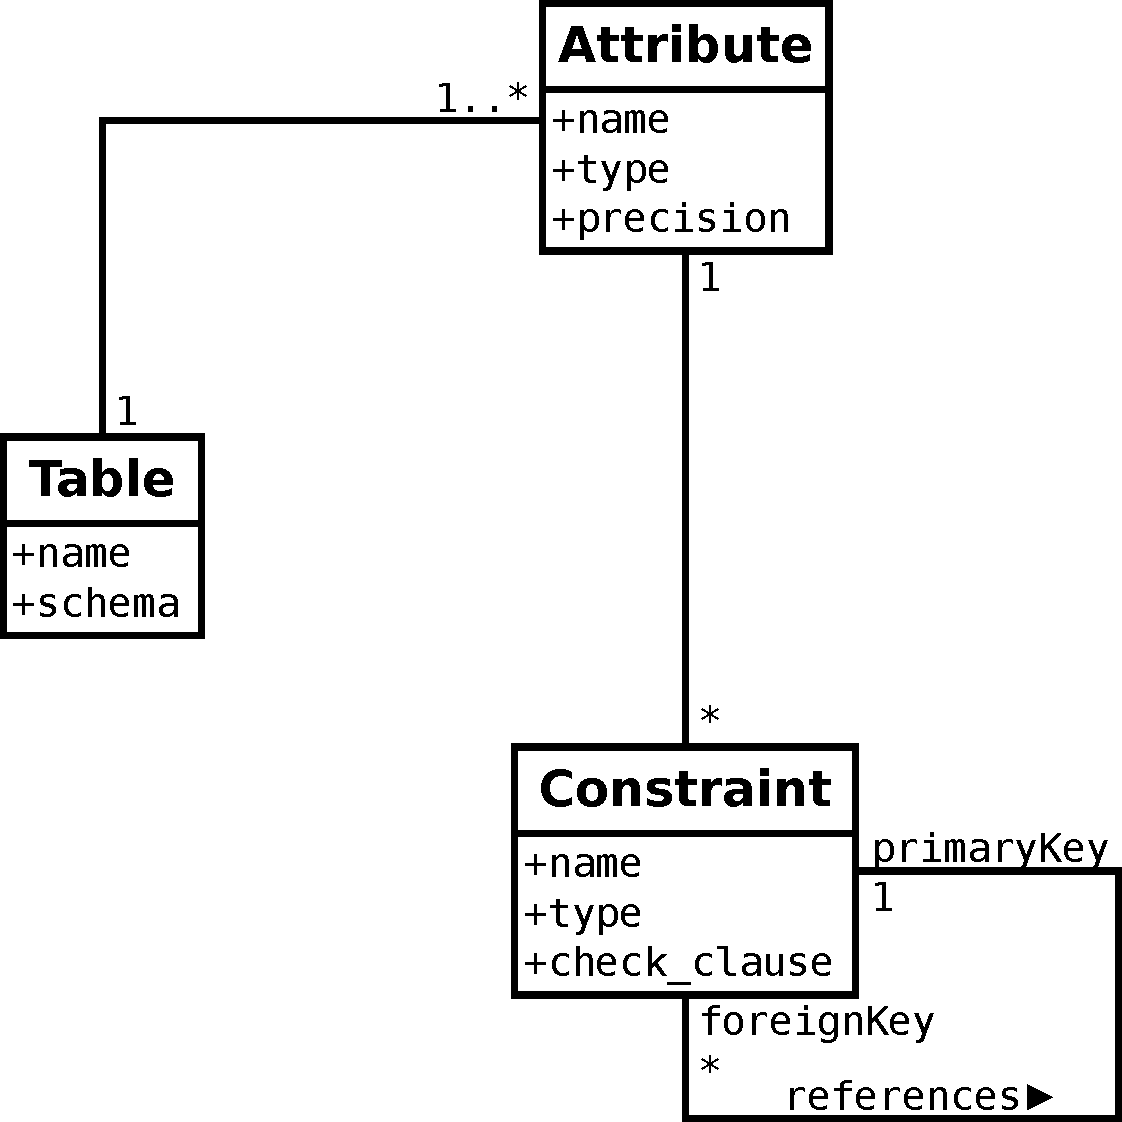
\includegraphics[width=0.6\textwidth]{files/diag_class_final}
\centering
\caption{Diagramme de classe représentant le modèle \emph{Hibernate}.}
\label{figure:diag_class_model_hibernate}
\end{figure}

\subsection{Paquet \texttt{conf.types}}
\label{subsection:conf.types}

Les types génériques sont définis dans des fichiers xml placés dans des sous paquets. A chaque type générique définis dans l'application, il suffit d'associer les types réels propres au SGBDR. 

Voici la DTD de ces fichiers de correspondance : 
\begin{verbatim}
<!ELEMENT genericTypes (genericType*)>
<!ELEMENT genericType (type*)>
<!ELEMENT type (#PCDATA) >

<!ATTLIST genericType name CDATA #REQUIRED>
\end{verbatim}


\subsection{Paquet \texttt{util}}
\label{subsection:util}

Dans ce paquet sont regroupé toutes les classes utilitaires non spécifique à l'application. 

\begin{description}
\item[OptionManager] Cette classe aide à la gestion des paramètres passé à une application.

\item[ImageFrame] Permet d'ouvrir facilement une fenêtre contenant une image.

\item[XmlUtil] Fournit une méthode pour parser des fichiers XML.
\end{description}



\section{Résultat}
\begin{frame}{Résultat}{Fonctionnalités implémentées}
\begin{itemize}
\item Fonctionnel sous Postgresql \& Mysql
\item Export du schéma sous de multiples formats
\textit{\scriptsize
\begin{tabular}{l l l l l l}
canon&cmap&cmapx&cmapx\_np&dot&eps \\
fig & gd & gd2 & gif & gv & imap \\
imap\_np & ismap & jpe & jpeg & jpg & pdf \\
plain & plain-ext & png & ps & ps2 & svg \\
svgz & tk & vml & vmlz & vrml & wbmp \\
x11 & xdot & xlib & & & \\
\end{tabular}}
\end{itemize}
\end{frame}

\begin{frame}{Résultat}{Schéma de sortie}
\begin{center}
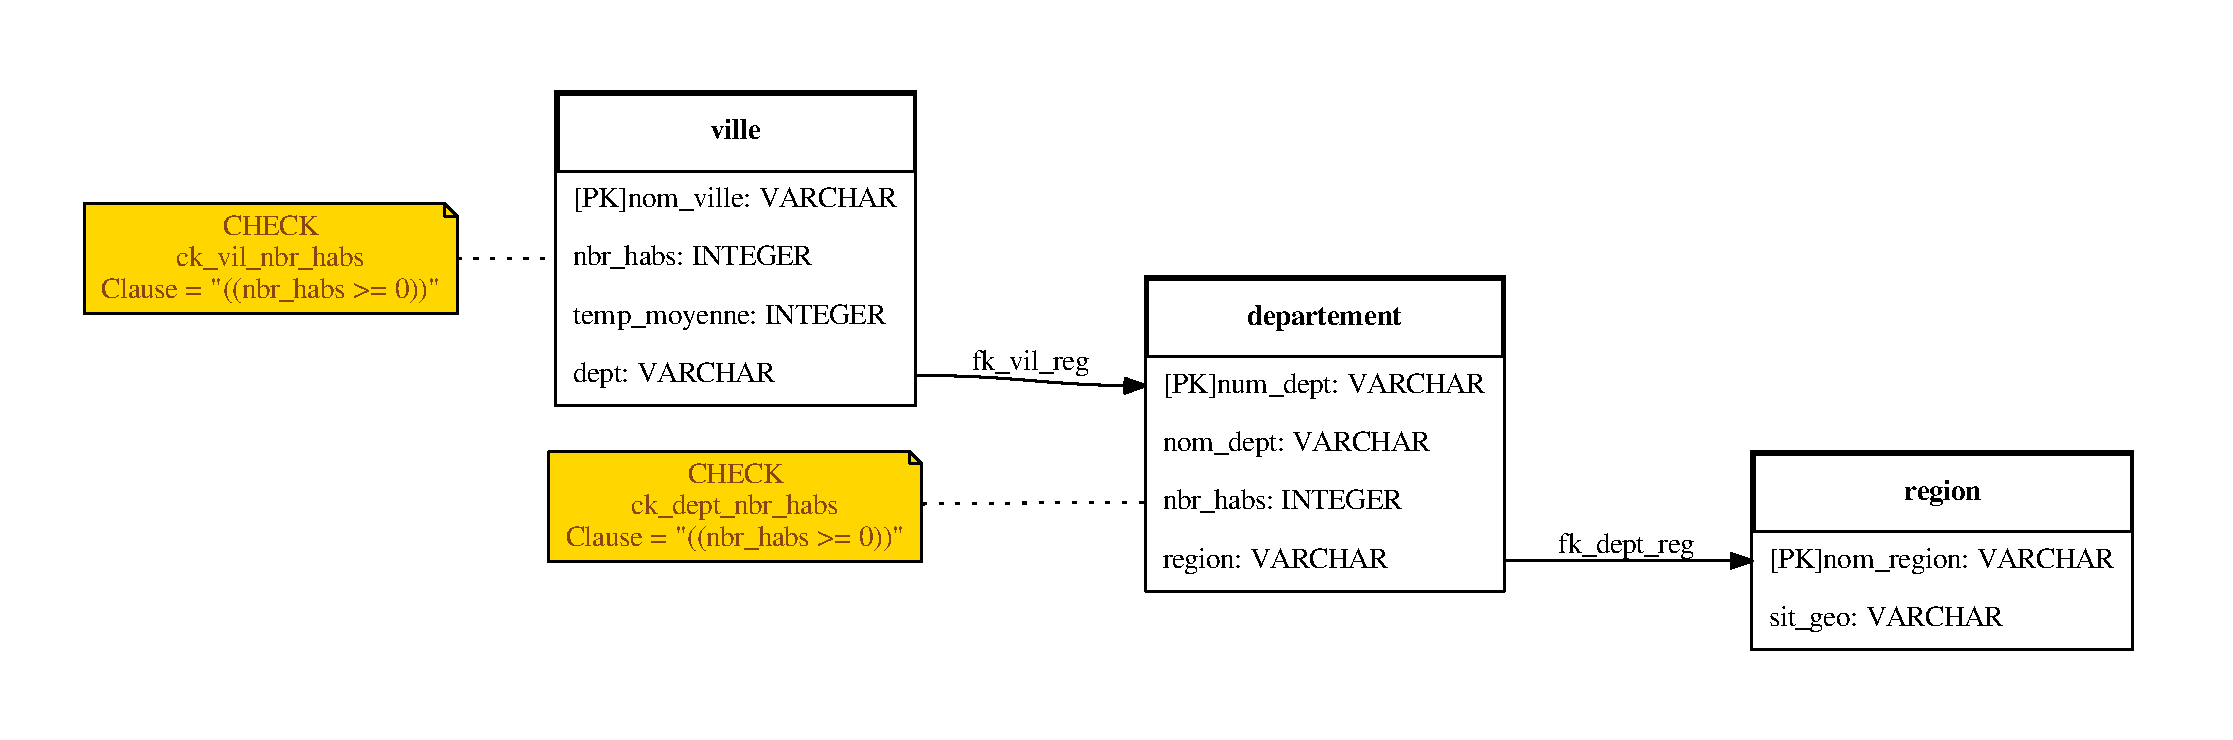
\includegraphics[width=\textwidth]{files/exemple_sortie}
\end{center}
\end{frame}

\end{document}
